\chapter{Evaluation of the Model Editor} \label{Evaluation_of_the_Model_Editor}
In this chapter, the created editor is evaluated. It is checked whether the requirements defined at the beginning have been successfully implemented. For this purpose, components of the editor such as the user interface, the visual syntax of the models or the code generator are examined more closely. Finally, a conclusion is drawn.

\section{Result of the Editor Development}
In this section it is checked whether the developed editor has fulfilled the requirements specified at the beginning.
\subsection{User Interface Evaluation}

Fig. \ref{fig:User_Interface} shows a screenshot of the user interface of the created SCCharts editor. In the centre is the SCChart model, which can be edited and customised. By clicking on elements in the editor, the \textsc{Cinco} properties are displayed in the lower area and can thus be adjusted. On the right, the SCChart components are clearly listed by type. These can be dragged and dropped into the model and the appropriate containers. Highlighting indicates whether the container can accommodate the component being created. Transitions can also be created by dragging and dropping. Superstates and root states can be resized and the regions and declarations they contain are adjusted accordingly. When declarations actions or suspensions are created, they are placed in the upper right area of the state, in which they are added. The regions are arranged correctly in the states when they are created. In addition, new SCCharts can be created and existing ones accessed via the project tree in the left-hand pane. This makes the editor a good user experience.

\begin{figure}[h!]
\centering
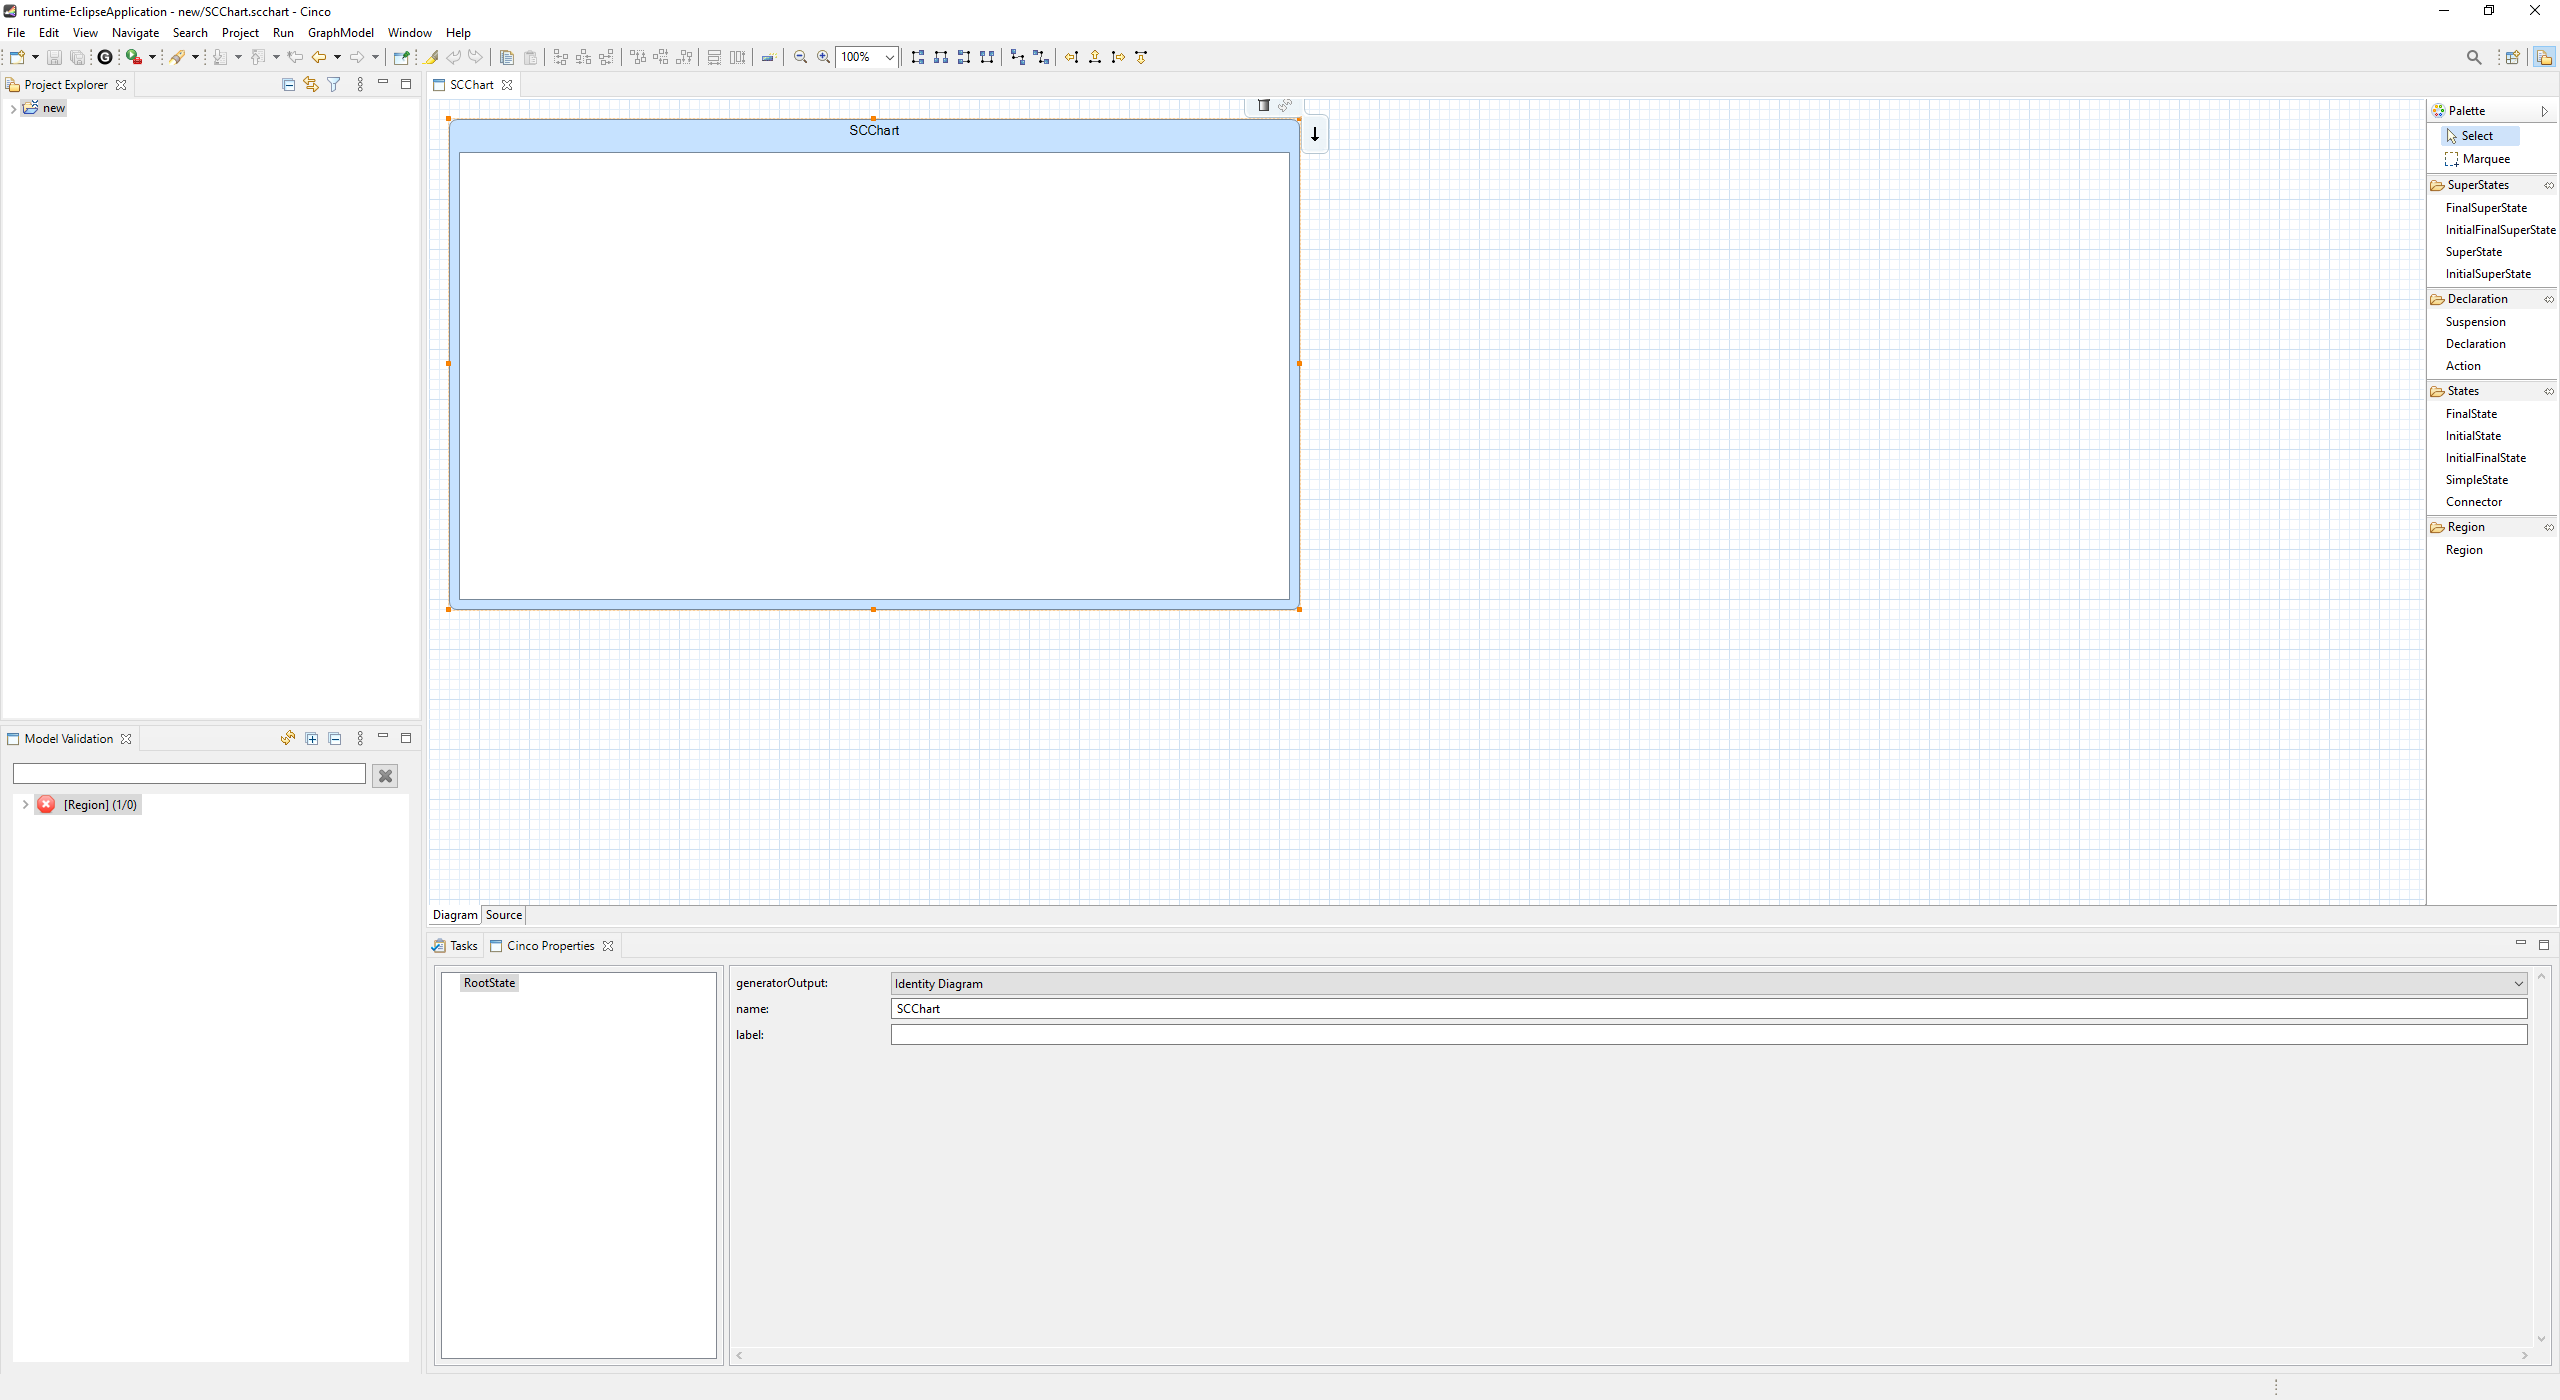
\includegraphics[width=1.0\textwidth]{bilder/User_Interface.png}
\caption{User Interface of the created SCChart Editor}
\label{fig:User_Interface}
\end{figure} 

\subsection{Visual Syntax Evaluation}

In Fig. \ref{fig:SCChartOverview_Comparison}, the upper part shows the SCCharts Overview image of Sect. \ref{Sequentially_Constructive_Statecharts} but without labels. Almost all the features of SCCharts can be seen in this picture. Below that is an SCCharts model created using the editor developed in this bachelor thesis, with a design similar to the \textit{SCCharts\_Overview} image. It can be clearly seen that these are almost identical models. Only the host code, which is declared last in fourth place in the root state in the original SCChart, is missing in the lower SCChart model. In addition, the priorities are indicated for components with only one outgoing transition, while these are not shown in the original SCChart. With deferred history transitions, the red circle of deferred is covered by the black circle of history. This is because only relative values can be assigned to the decorators and therefore no fixed distance to the end of the arrow is possible. In addition, the Appearance Provider plug-in changes the entire appearance in the style so that, for example, the line of the green triangle is also dashed for the termination transition. Nevertheless, these are only minor deviations. All in all, the components of SCCharts are clearly recognisable.

\begin{figure}[h!]
\centering
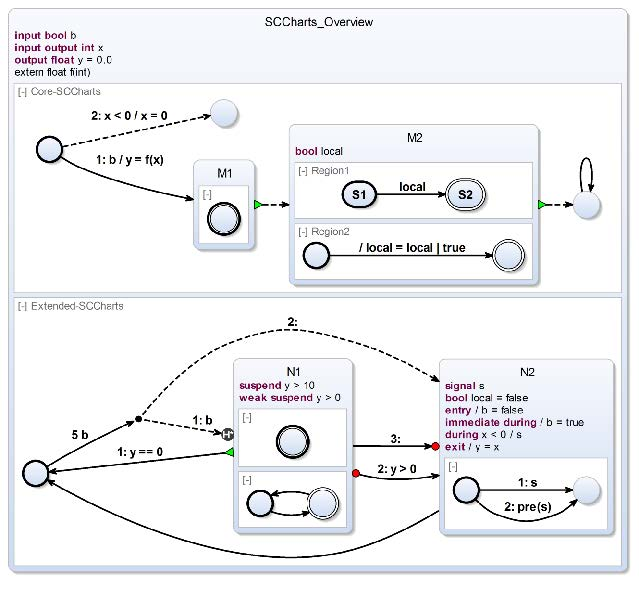
\includegraphics[width=0.9\textwidth]{bilder/SCCharts_Overview_Without_Declarations.jpg}
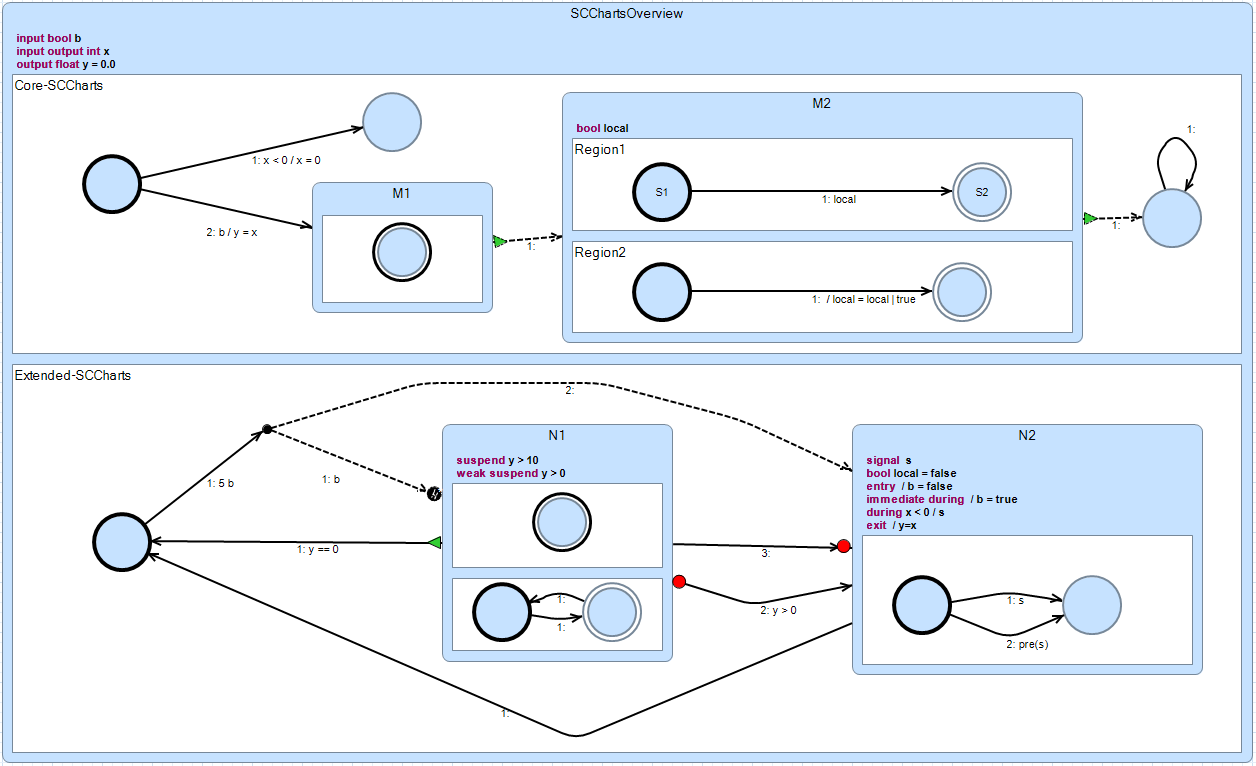
\includegraphics[width=0.9\textwidth]{bilder/CincoSCChartOverview.png}
\caption{Original SCCharts model (top) and editor SCChart model (bottom)}
\label{fig:SCChartOverview_Comparison}
\end{figure} 

\subsection{Validation Evaluation}

A validation was implemented via the MCaM plugin, which performs checks after saving the model. For a better overview and easier extension, a separate check class was created for each class or superclass of components of the MGL. Several validation functions are implemented.

Fig. \ref{fig:ValidationExample} shows some examples of validation functions. In the middle is a model with incorrect syntax. The validations are shown at the bottom left. The first error indicates that the order of outgoing transitions from an initial state, state A, is not valid. This is because both transitions originating from A have priority 1. Next, it indicates that a region does not contain exactly one initial state. This is the case in the second region of the superstate. And the last error message displayed is that for a transition, source and target are not in the same region, which is the transition from A to B. 
\begin{figure}[h!]
\centering
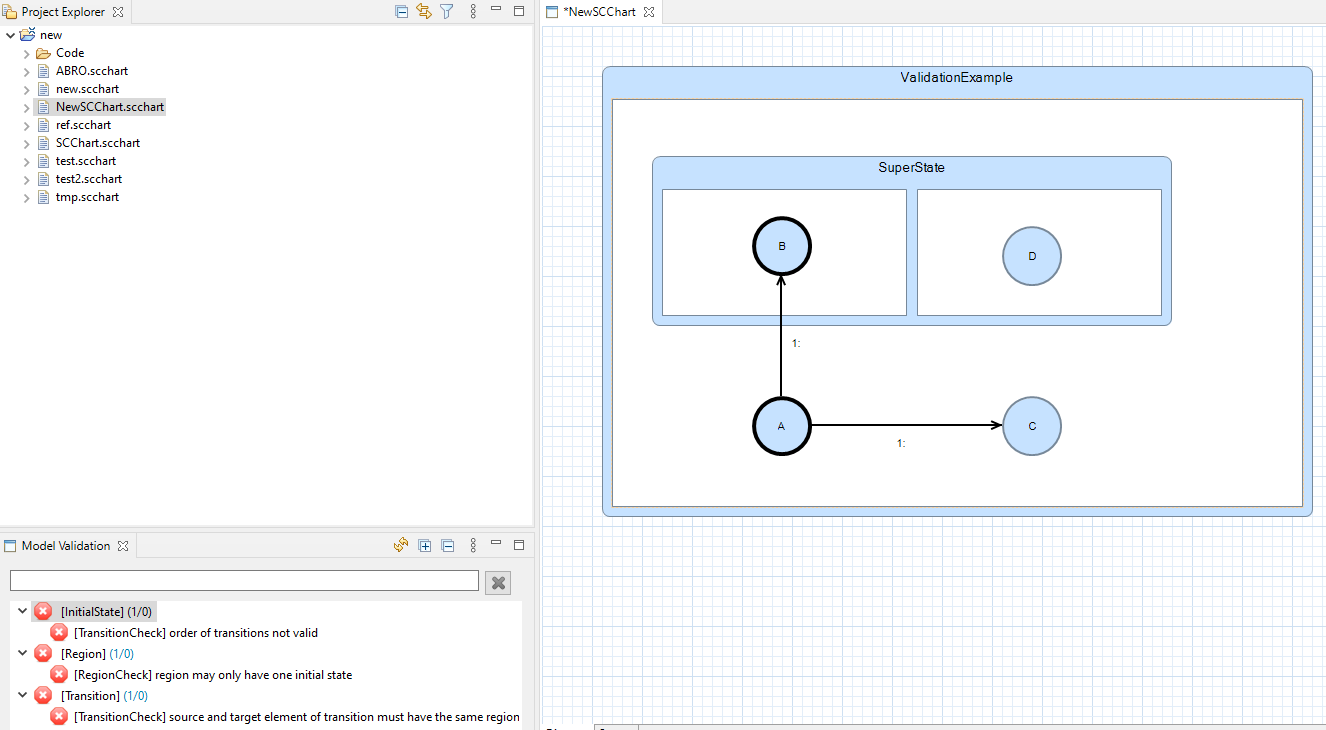
\includegraphics[width=1.0\textwidth]{bilder/CincoValidationExample.png}
\caption{Example for MCaM plugin for SCChart Validation}
\label{fig:ValidationExample}
\end{figure} 

\subsection{Code Generator Evaluation}

Through \textsc{Cinco}'s code generator meta plugin it is possible to start the code generation by clicking the generate button in the user interface. This translates the currently opened model into SCT and saves it in a file in the workspace. In addition, the KIELER SCCharts CLI is started via the command line. This takes the file in SCT format as input, and a parameter selected by the user via the root state that defines the target language of the output. This can be C or Java code, but also a SCChart diagram, which provides the possibility to compare the with the editor created SCChart model with that one of the KIELER SCChart CLI. In this way, the created model can be checked again to make sure that it meets the original requirements. In the context of this bachelor thesis, this is mainly useful to check if the code generator interprets the components of the model correctly.

An example of the output of the implemented code generator is presented in Fig. \ref{fig:CINCO_CodeGenerator}. It shows the ABRO SCChart, the "hello world" of synchronous programming~\cite{Hanxleden.2014}. Here are the functions of concurrency and preemption illustrated in a compact example. At the top left is the SCChart model from the developed \textsc{Cinco} SCChart Editor. The input and output booleans are listed in the upper section of ABRO. The strong abort transition of ABO leads to the fact that if input R is true, ABO is immediately reset, the preempt function. Within ABO, another initial superstate with 2 regions to represent concurrency, is shown. The diagram of the KIELER SCCharts CLI (bottom right) can be seen as relatively identical, as the components only differ slightly by position. This means that both the SCT code (top right) and the Java code (bottom left) created from the model (top left) with the code generator of the \textsc{Cinco} SCChart editor can be considered correct. 

However, if the model created with the SCChart editor is incorrect, the code generator also creates an incorrect SCT file, which cannot be processed by the KIELER SCCharts CLI, so that neither Java or C code nor a diagram is generated. This can also happen if, for example, a variable is specified in a condition that does not exist in the model. This allows the tool to be improved in one or two places. Nevertheless, the code generator already works quite reliably.
\begin{figure}[h!]
\centering
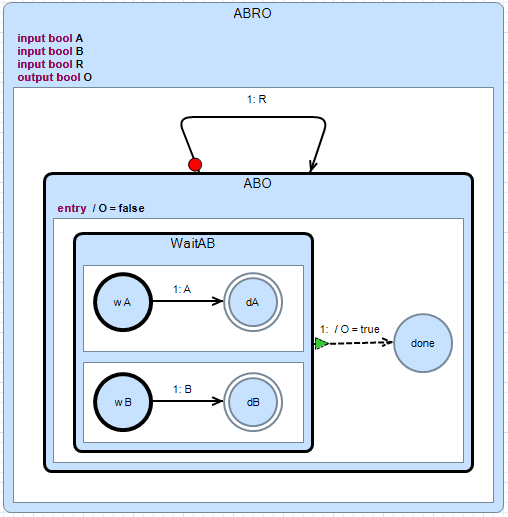
\includegraphics[width=0.5\textwidth]{bilder/CincoABROModel.png}
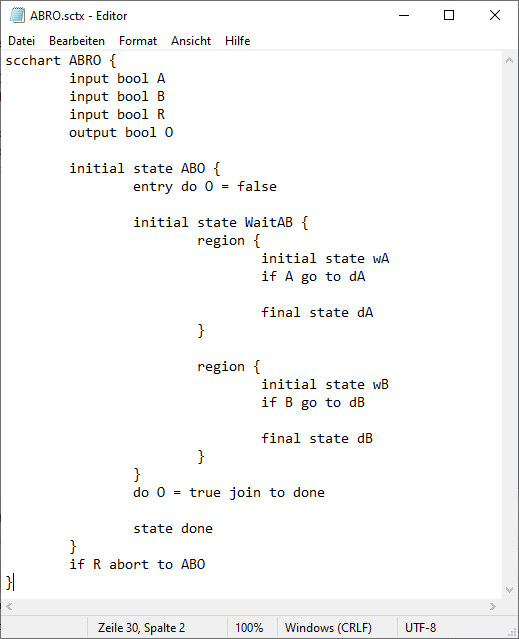
\includegraphics[width=0.43\textwidth]{bilder/ABRO_SCT.png}
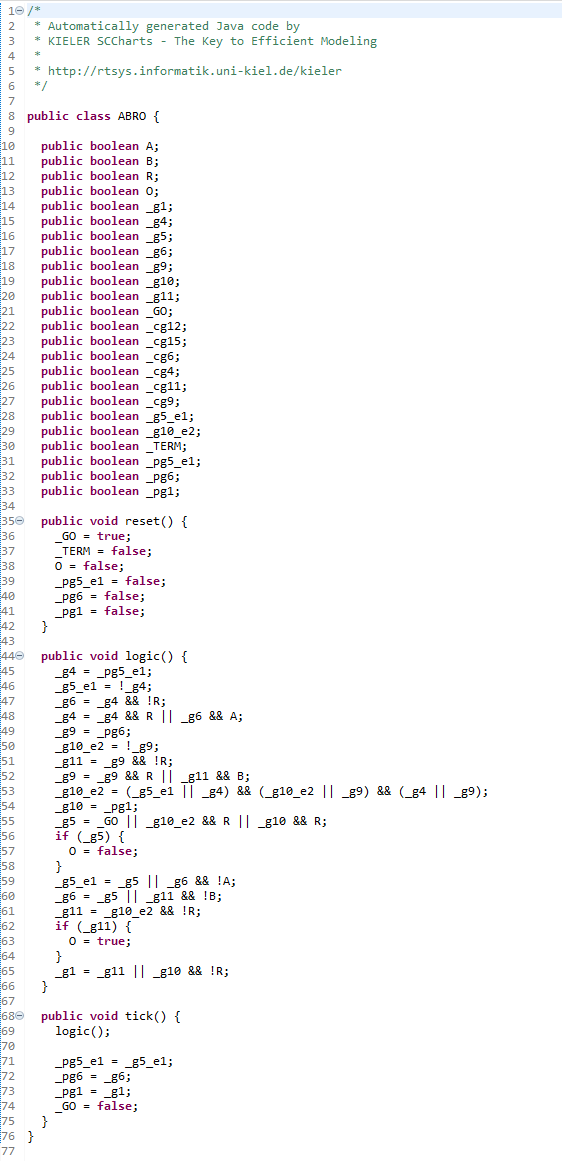
\includegraphics[width=0.35\textwidth]{bilder/ABROJavaCode.png}
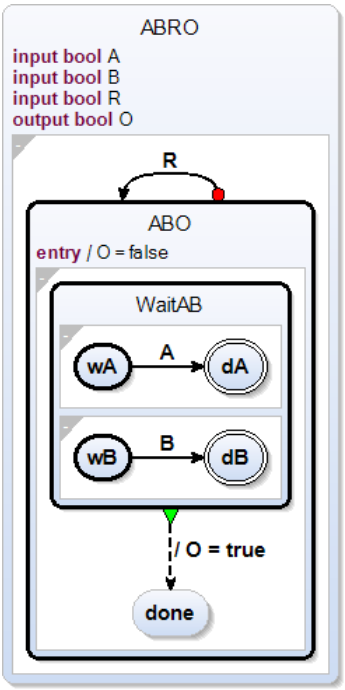
\includegraphics[width=0.38\textwidth]{bilder/ABROIdentityDiagram.png}
\caption{Output of the code generator plug-in from the ABRO SCChart}
\label{fig:CINCO_CodeGenerator}
\end{figure} 
\section{Conclusion}
With the conception and implementation of a domain specific graphical tool it should be shown that its development does not have to be tedious and complex as often assumed. The Cinco meta tool was the perfect tool for this, as it can be used to create graphical DSL tools, and its main feature is its full generation from meta specifications. This means that tools generated by cinco can be executed directly without having to adapt the code as is the case with other meta tools with semi-automatic generation. In general, cinco follows a simplicity-driven approach that imposes restrictions in order to avoid complexity.

As the graphical DSL the SCCharts language was chosen, which was designed to be used as a visual modeling language for safety-critical applications. These bring with them a wide range of features, many of which were realised in the editor that was finally developed. On the basis of previously defined requirements and a data structure containing all the important components and associations of the SCChart language that should be included in the editor, the implementation of the editor's MGL was started. Through the preliminary work with the data structure, the implementation of the MGL could be completed quickly. The SGL was oriented as closely as possible to the visual syntax of SCCharts. As a result, the visual representation of components was limited to the runtime of Cinco. Since every small difference in the visual representation can almost only be implemented by defining a new component in the MGL with its own style, which meant that many transitions of SCCharts differing only slightly still had to be defined in the MGL as own component. However, the Appearance provider, which allowed a few changes to be made at runtime, reduced the number of transitions to be defined in the MGL. After MGL and SGL were implemented, SCCHart models could be created, but it was neither intuitive nor dynamic, as all lay-outing was left to the user and the interface was not very user-friendly. The various cinco meta-plugins made it easy to modify the interface of the editor and adapt it to the DSL. They also provide a large number of functions that improve the layout of the SCChart model and thus make it possible to create more dynamic and improved models. Subsequently, the generation of integrable java and c code from the models created with the Cinco SCChart editor was realised via a further plug-in from Cinco and with the help of an SCChart compiler tool. Subsequently, the generation of integrable java and c code from the models created with the Cinco SCChart editor was realised via a further plug-in from Cinco and with the help of an SCChart compiler command line interface. The evaluation of the editor has shown that although it is not yet perfect, it is already a great support for the graphical creation of SCChart models. And the code generator is already a very useful tool. 

All in all, it was shown that a powerful and useful tool for modelling DSLs can be developed with relatively little effort. In addition, the cinco meta tool has shown that it can be used both for DSLs that offer many features and for DSLs in the security-critical area.